\clearpage

\section{graphNVP}\label{sec:graphNVP}\index{graphNVP}

\begin{notebox}
\textbf{Paper: } \fullcite{madhawa_graphnvp_2019}
\vspace{5pt}

\href{https://openreview.net/forum?id=ryxQ6T4YwB}{ICLR not accept reviews}
\hspace{1cm}
\href{https://github.com/pfnet-research/graph-nvp}{Official code}
\hspace{1cm}
\href{run:/home/magda/Dropbox/Zot/Madhawa et al_2019_GraphNVP.pdf}{Local pdf}

\hfill Notes taken: 6/2/2022 \index{February 2022}
\end{notebox}

\begin{notebox}[colback=red!5]
\tldr Generate graphs\index{graph} $G = (A, X)$ through invertible flows\index{invertible flow}. Dequantize\index{dequantize} A and X by uniform noise to make modelling continuous. Coupling strategy splitting the A and X matrices always by one node vs all the rest (breaks permutation invariance). The scale and translation in the coupling are graph NNs (do not have to be invertible) - for X functions of all other nodes and complete A matrix; for A edges between other nodes. Final reconstructed / generated A, X are quantized (floored) to get back to discrete.
\end{notebox}

\begin{notebox}[colback=yellow!5]
\textbf{Notes:} 
\begin{itemize}[nosep]
\item Dequantize by simple uniform noise to get rid of the discreteness problem, then simply quantize (floor) to get back.
\item ZINC-250K random sample of 250k molecules from complete ZINC to make experiments manageable. 
\item Good list of baseline models for experiments
\item No validation checks during generation $\to$ versatile and fast.
\item Coupling structure by nodes breaks permutation invariance - is this really a problem?
\end{itemize}
\end{notebox}

\begin{figure}[ht]
\centering
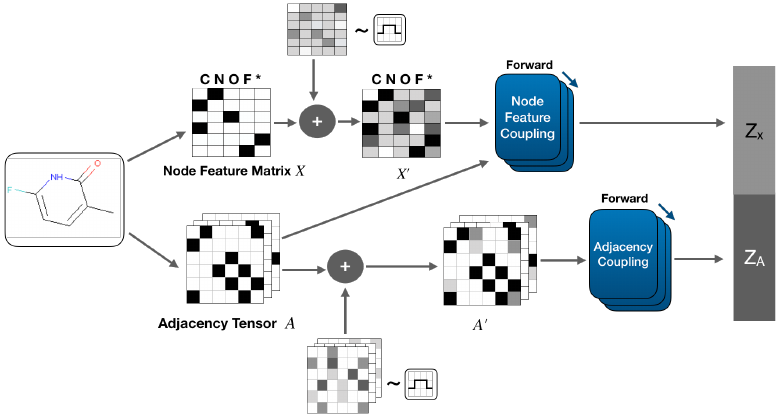
\includegraphics[width=10cm]{graphNVP_Figure1.png}
\caption{For the forward transform, A and X matrices are perturbed by uniform noise. The node coupling is conditioned on the A matrix.}
\end{figure}

\begin{figure}[ht]
\centering
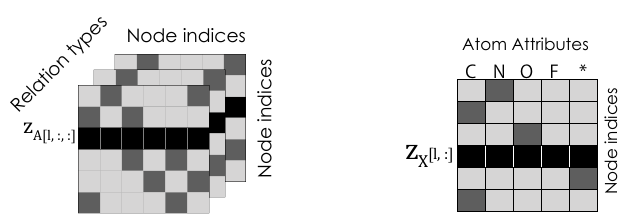
\includegraphics[width=6cm]{graphNVP_Figure2.png}
\caption{The coupling structure splits the A and X matrices as one node vs all the rest. This works best in experiments, though breaks down permutation invariance.}
\end{figure}

\begin{figure}[ht]
\centering
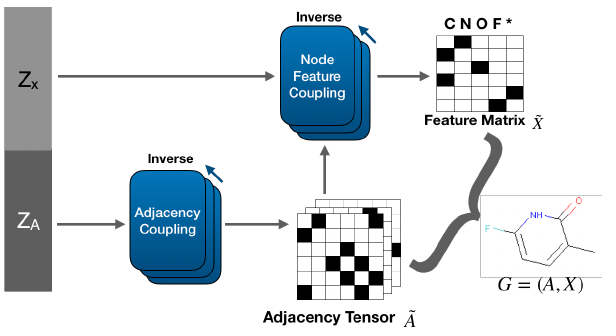
\includegraphics[width=8cm]{graphNVP_Figure3.png}
\caption{Generation is in two steps because the reverse coupling transform of X is conditioned on A so this needs to be generated first. Using simple dequantization (flooring) to get from continuous flow output to discrete A, X.}
\end{figure}

\textbf{Experiments:} on QM9\index{QM9} and ZINC-250K\index{ZINC} with kekulized graphs (without hydrogens) - our \emph{cheat} version.
Have not so great validity but high uniqueness.
Claim benefits in speed of generation as opposed models that have complex decoders checking the validity of molecules in the process.
Some comments on smoothness of latent space and possibility to interpolate for property control but not very convincing.
